%論理回路の入出力方法
\section{論理回路の入出力方法}

もしあなたが人間ならば、実際に電子工作で論理回路で何かを作成したときに、人間が論理回路に信号を与えてあげる入力と、人間が論理回路からの信号を受け取る出力が必要になるだろう。

\subsection{出力方法}
まず、論理回路の出力としてLEDを使うのが最もわかりやすい方法である。
A=HighのときにLEDが点灯し、A=LowのときにLEDが消灯するようにするには図\ref{fig:led_output_source}と図\ref{fig:led_output_sink}の2通りの方法がある。
\begin{figure}[htbp]
    \begin{minipage}
        {0.45\hsize}
        \centering
        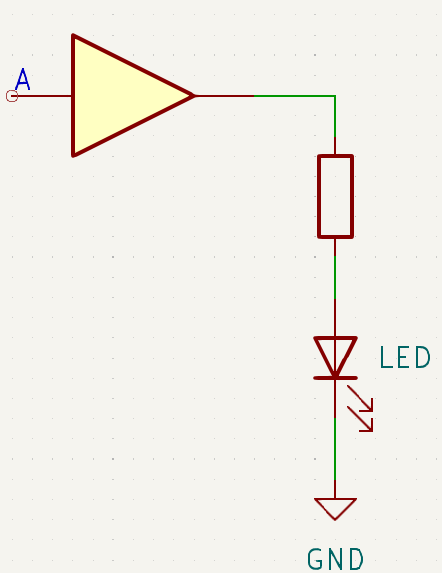
\includegraphics[width=0.6\textwidth]{apply/led_output_source.png}
        \caption{LEDをソース側に接続した出力回路}
        \label{fig:led_output_source}
    \end{minipage}
    \begin{minipage}
        {0.45\hsize}
        \centering
        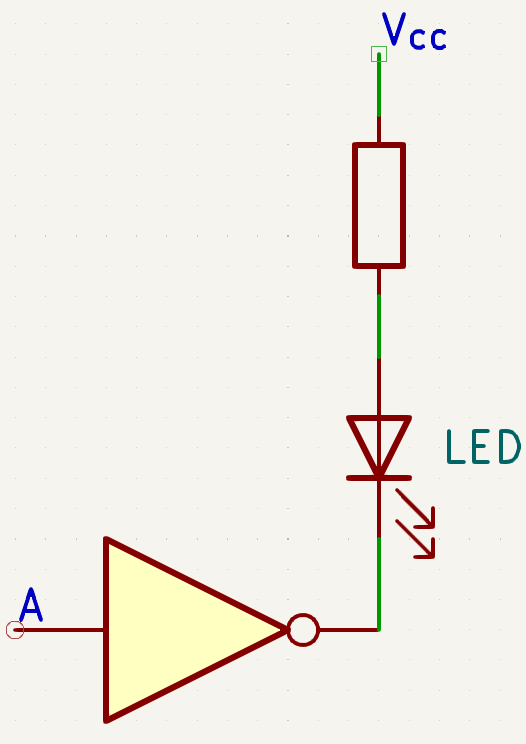
\includegraphics[width=0.6\textwidth]{apply/led_output_sink.png}
        \caption{LEDをシンク側に接続した出力回路}
        \label{fig:led_output_sink}
    \end{minipage}
\end{figure}
図\ref{fig:led_output_source}の回路では、論理回路の出力がHighのときに論理回路からLEDに電流が流れ、LEDが点灯する。
一方、図\ref{fig:led_output_sink}の回路では、論理回路の出力がLowのときに$V_{cc}$からLEDに電流が流れ、LEDが点灯する。
このように、どちらの方法でもLEDを点灯させることができる。

74HCシリーズの場合、論理回路が流せる電流は最大で約20mAであり、LEDが点灯するために必要な電流は約5～10mAであるため、直接LEDを接続しても問題ない。
しかし、LEDではない出力装置を使う場合や、複数のLEDを接続する場合などは、論理回路から直接電流を流すことができない場合がある。
その場合は、トランジスタを用いて論理回路の出力を増幅する必要がある。
図\ref{fig:transistor_output_emitter_ground},\ref{fig:transistor_output_emitter_follower}にトランジスタを用いた出力回路の例を示す。

\begin{figure}[htbp]
    \begin{minipage}
        {0.45\hsize}
        \centering
        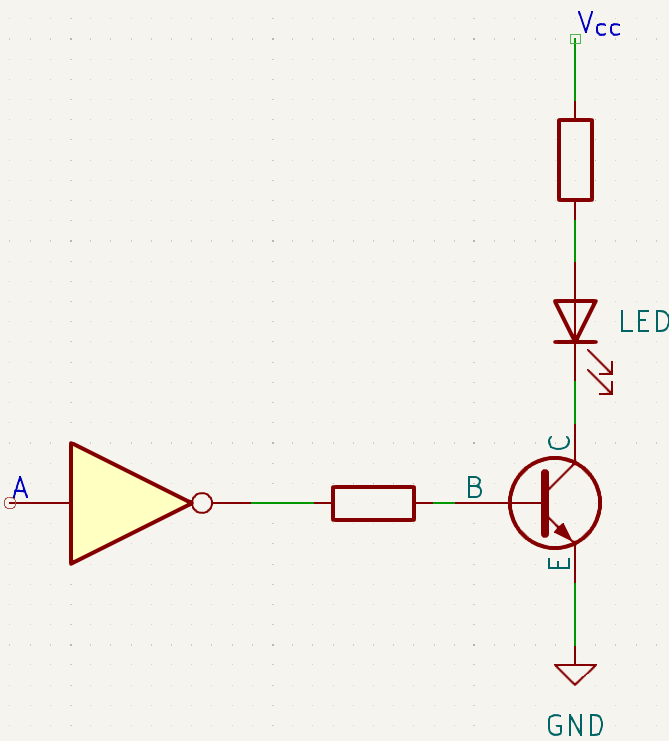
\includegraphics[width=0.8\textwidth]{apply/transistor_output_emitter_ground.png}
        \caption{エミッタ接地回路を用いた出力回路}
        \label{fig:transistor_output_emitter_ground}
    \end{minipage}
    \begin{minipage}
        {0.45\hsize}
        \centering
        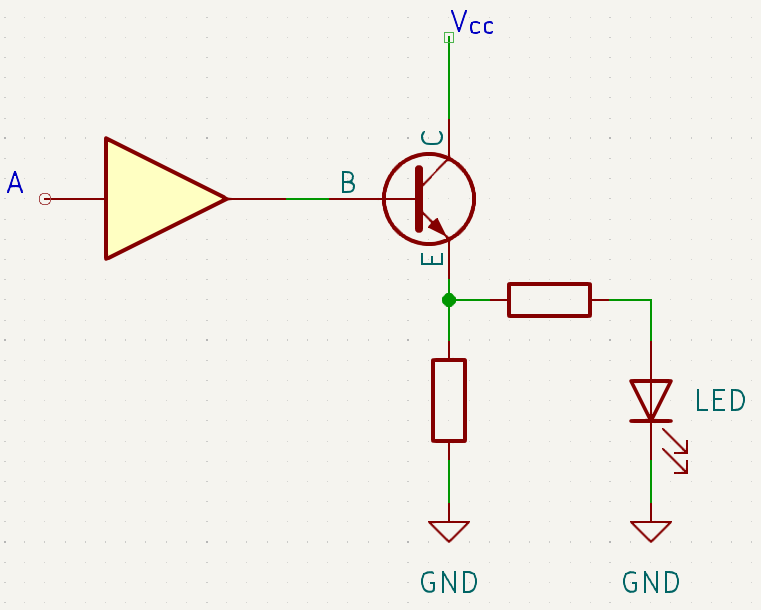
\includegraphics[width=0.95\textwidth]{apply/transistor_output_emitter_follower.png}
        \caption{エミッタフォロワ回路を用いた出力回路}
        \label{fig:transistor_output_emitter_follower}
    \end{minipage}
\end{figure}

\newpage

これらの回路を用いることで、論理回路の出力を増幅し、より大きな電流を流すことができる。

しかし、これらの回路には欠点が存在する。
トランジスタがONからOFFに切り替わるときに、トランジスタ内部に少数キャリアが過剰に残っているため、そいつらがキャリアとなり電流が流れなくなるまで時間がかかる。
この現象を少数キャリア蓄積効果と呼び、これによりスイッチング速度がおよそ3$\mu$s程度遅くなる。
このため、高速に動作させたい場合,図\ref{fig:transistor_output_emitter_ground_speedup}のような回路を用いる。
\begin{figure}[htbp]
    \centering
    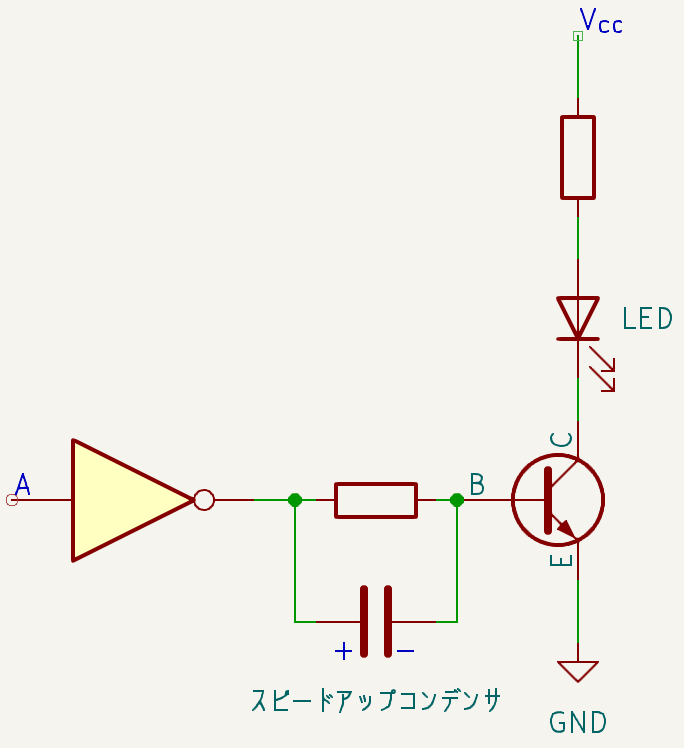
\includegraphics[width=0.5\textwidth]{apply/transistor_output_emitter_ground_speedup.png}
    \caption{スピードアップコンデンサを付けたエミッタ接地回路}
    \label{fig:transistor_output_emitter_ground_speedup}
\end{figure}
\newpage
この回路は100pF程度のコンデンサ(スピードアップコンデンサという)
を論理回路の出力とトランジスタのベースの間に接続することで、
論理回路の出力がHighの間に電荷を図の通りに蓄えて、Lowに切り替わったときに
その電荷を用いてベースに負の電圧をかけることで少数キャリアを強制的に排出し、スイッチング速度を向上させる回路である。

\subsection{入力方法}
論理回路に信号を入力する方法として、最も簡単な方法はスイッチを用いる方法である。
ここで図\ref{fig:switch_gate_fail1}のようにゲートにスイッチを接続したくなるが、この方法は正しく動作しない。
\begin{figure}[htbp]
    \begin{minipage}
        {0.45\hsize}
        \centering
        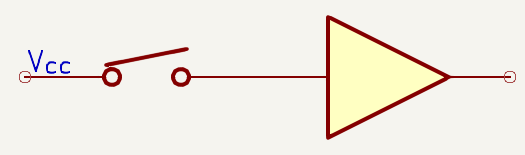
\includegraphics[width=0.6\textwidth]{apply/switch_gate_fail1.png}
        \caption{ゲートへのスイッチ接続例(誤1)}
        \label{fig:switch_gate_fail1}
    \end{minipage}
    \begin{minipage}
        {0.45\hsize}
        \centering
        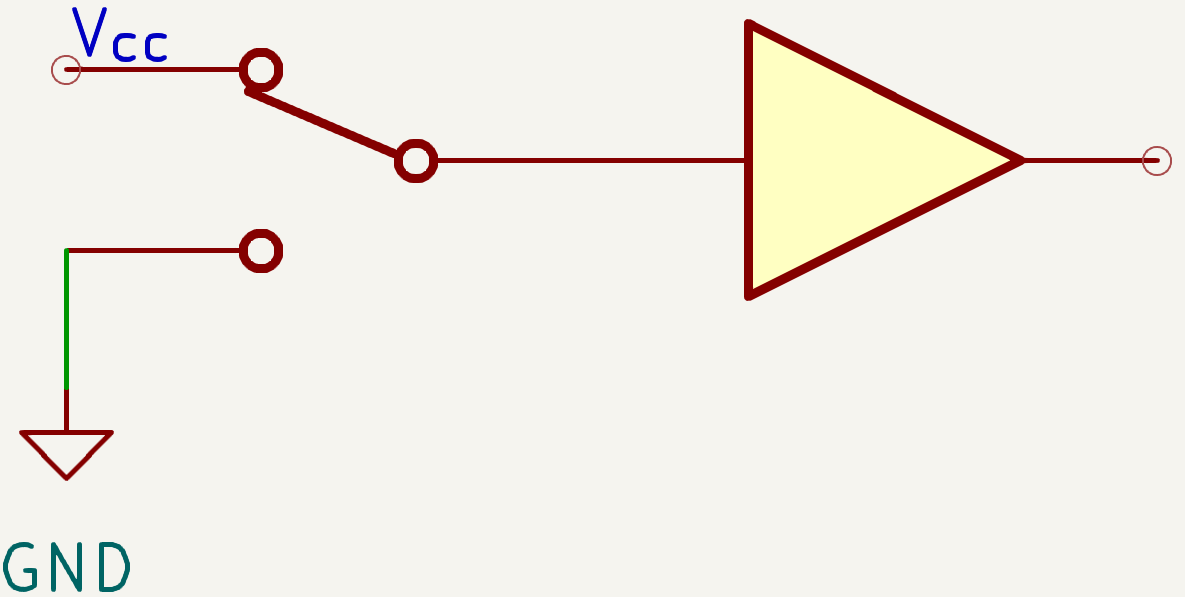
\includegraphics[width=0.6\textwidth]{apply/switch_gate_fail2.png}
        \caption{ゲートへのスイッチ接続例(誤2)}
        \label{fig:switch_gate_fail2}
    \end{minipage}
\end{figure}
なぜならば、このスイッチを開いた場合に、論理回路の入力が浮遊状態となり、不定の電圧となってしまうため、動作が保障されない。

図\ref{fig:switch_gate_fail1}の回路がだめならば、図\ref{fig:switch_gate_fail2}のようにスイッチでGNDと$V_{cc}$を切り替えればうまくいくかもしれないと考えるかもしれないが
、この方法も上手くいかない。
なぜならばスイッチはどちらかの接点と離れたタイミングと全く同じ時間にもう一つの接点と接続されるわけではないためである。
まず、切り替え時に両方の接点と離れてしまう場合(Break-Before-Makeという)、論理回路の入力が浮遊状態となり、不定の電圧となってしまうため、動作が保障されない。
一方、切り替え時に両方の接点と接続されてしまう場合(Make-Before-Breakという)、論理回路の入力が一瞬であるが短絡状態となってしまい、過大な電流が流れてしまう可能性があるため、危険である。
\newpage
このように、スイッチを用いて論理回路に信号を入力する場合は、プルアップ抵抗またはプルダウン抵抗を用いて、スイッチが開いたときに論理回路の入力が浮遊状態にならないようにする必要がある。
図\ref{fig:switch_gate_pullup}にプルアップ抵抗を用いたスイッチ接続例を、図\ref{fig:switch_gate_pulldown}にプルダウン抵抗を用いたスイッチ接続例を示す。
\begin{figure}[htbp]
    \begin{minipage}
        {0.45\hsize}
        \centering
        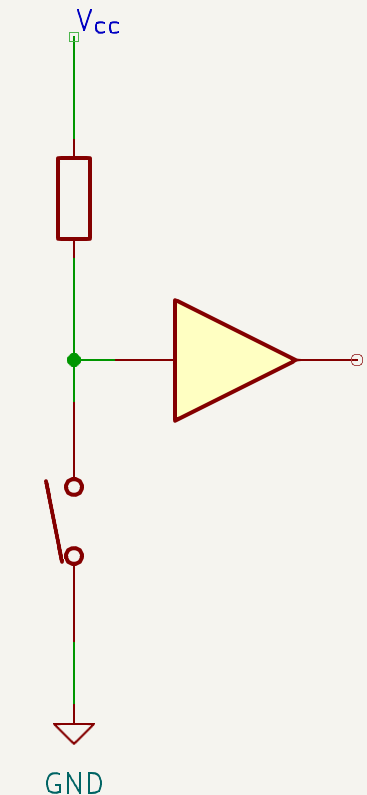
\includegraphics[width=0.6\textwidth]{apply/switch_gate_pullup.png}
        \caption{プルアップ抵抗を用いたゲートへのスイッチ接続例}
        \label{fig:switch_gate_pullup}
    \end{minipage}
    \begin{minipage}
        {0.45\hsize}
        \centering
        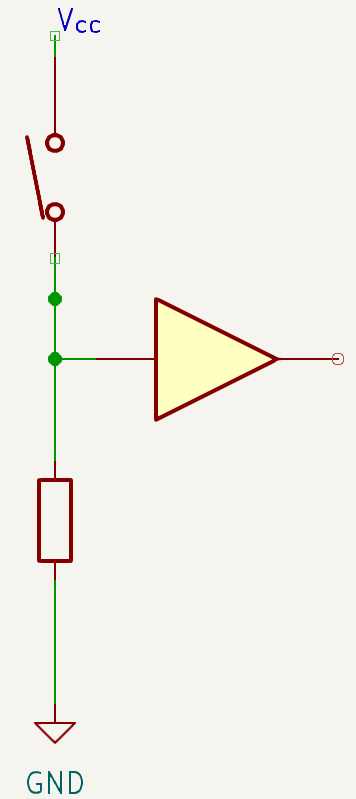
\includegraphics[width=0.6\textwidth]{apply/switch_gate_pulldown.png}
        \caption{プルダウン抵抗を用いたゲートへのスイッチ接続例}
        \label{fig:switch_gate_pulldown}
    \end{minipage}
\end{figure}
図\ref{fig:switch_gate_pullup}の回路では、スイッチが開いているときにプルアップ抵抗によって論理回路の入力が$V_{cc}$に引っ張られ、高電位(H)となる。
一方、スイッチが閉じているときに論理回路の入力がGNDに接続され、低電位(L)となる。
プルダウンの回路も同様に動作する。
このように、スイッチを用いて論理回路に信号を入力する場合は、プルアップ抵抗またはプルダウン抵抗を用いて、スイッチが開いたときに論理回路の入力が浮遊状態にならないようにする必要がある。

プルアップ、プルダウン抵抗の抵抗値は、通常数k$\Omega$から数十k$\Omega$程度が用いられる。

しかし、スイッチを使う際に注意しなければならない点がある。
スイッチを押したときに、接点がバウンドし、チャタリングと呼ばれる現象が発生することがある。
チャタリングが発生すると、スイッチを一回押しただけで、論理回路の入力がHighとLowを何度も繰り返すことになり、正しく動作しない可能性がある。
このチャタリングをはソフト的な対策を行うこともできるが、最も簡単なハード的対策として、図\ref{fig:switch_debounce}のようなチャタリング防止回路を用いることができる。
\begin{figure}[htbp]
    \begin{minipage}
        {0.45\hsize}
        \centering
        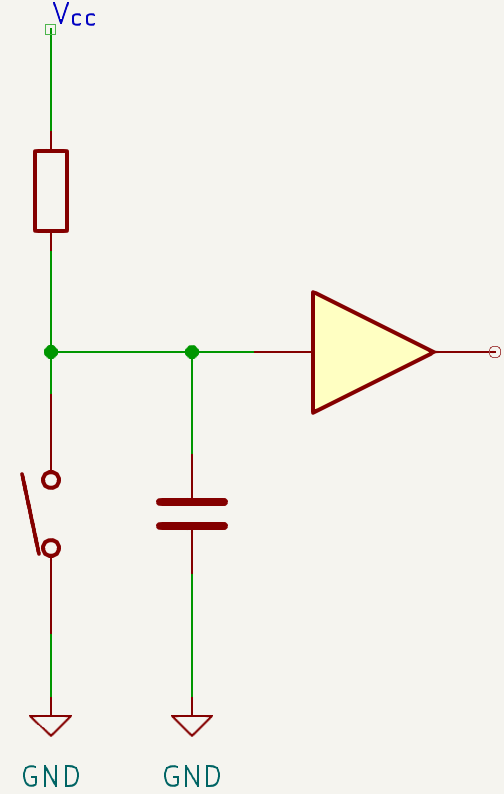
\includegraphics[width=0.7\textwidth]{apply/switch_debounce.png}
        \caption{チャタリング防止回路の例}
        \label{fig:switch_debounce}
    \end{minipage}
    \begin{minipage}
        {0.45\hsize}
        \centering
        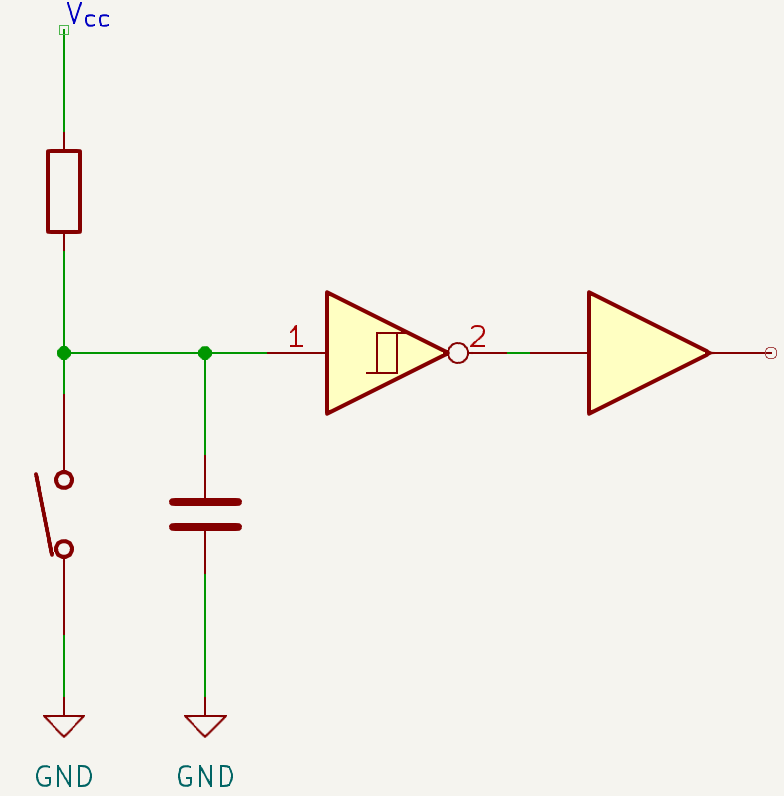
\includegraphics[width=0.9\textwidth]{apply/switch_debounce_schmitt.png}
        \caption{シュミットトリガ回路を組み合わせたチャタリング防止回路の例}
        \label{fig:switch_debounce_schmitt}
    \end{minipage}
\end{figure}

この回路ではチャタリングが発生しても、コンデンサ$C_1$が充放電を行うことで、論理回路の入力に加わる電圧がゆっくりと変化するようになり、チャタリングの影響を受けにくくなる。
しかし、この回路の問題点として、例えば、ONからOFFに切り替わったときに、コンデンサ$C_1$が充電される過渡応答が発生するが、
そのゆっくりとした過渡応答で、論理回路がHighとみなす電圧とLowとみなす電圧付近を行ったり着たりすることがあり、論理回路の動作がバタつく。
そのため、この回路にシュミットトリガ回路という、入力電圧がある閾値を超えたときにのみ出力が切り替わる回路を組み合わせることで、より安定した動作を実現できる。(図\ref{fig:switch_debounce_schmitt}参照)
% \begin{figure}[htbp]
%     \centering
%     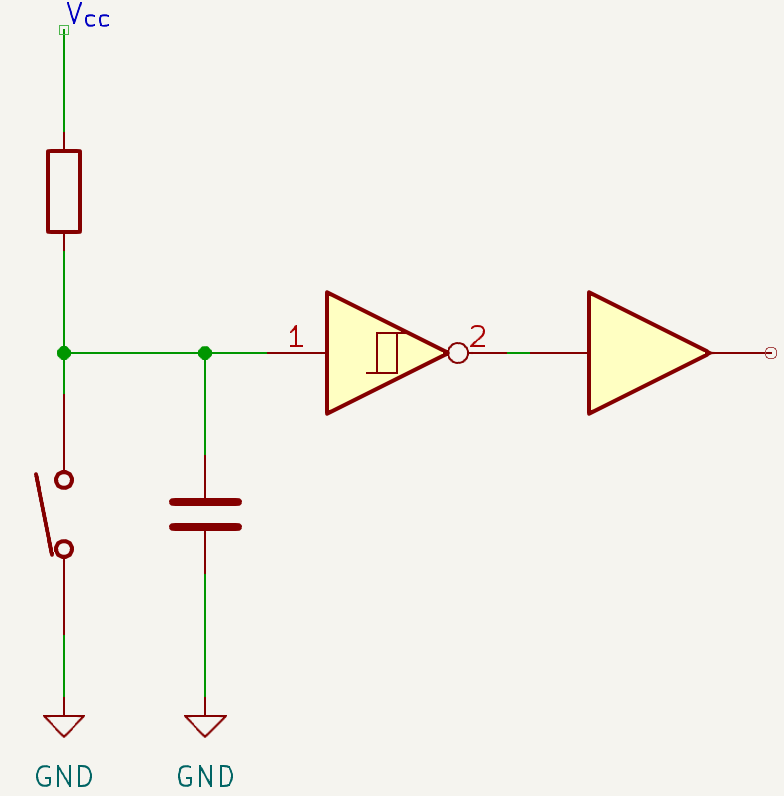
\includegraphics[width=0.6\textwidth]{apply/switch_debounce_schmitt.png}
%     \caption{シュミットトリガ回路を組み合わせたチャタリング防止回路の例}
%     \label{fig:switch_debounce_schmitt}
% \end{figure}
% \newpage

\section{未使用ピンの処理}
論理回路には未使用の入出力ピンが存在する場合がある。
例えば、74HC00は4つのNAND回路を1つのICに内蔵しているが、1つだけNAND回路を使用する場合、残りの3つのNAND回路の入力ピンは未使用となる。
このような未使用の入出力ピンをそのままにしておくと、心理的に不安である。

これらの処理方法を説明する。

未使用の入力ピンは、プルアップ抵抗またはプルダウン抵抗を用いて、論理回路の入力が浮遊状態にならないようにしておけば安心である。
プルアップかプルダウンのどちらを用いるかであるが、出力がLowになるように選ぶとよいとされているが、めんどくさいなら全部プルダウンでよい。

未使用の出力ピンは、基本オープンで大丈夫だが、
オープンコレクタ出力の場合だけは例外で、プルアップかプルダウンをしておく必要がある。
プルアップかプルダウンのどちらを用いるかであるが、消費電力を下げるほうを選ぶとよいとされている。

